% New, separately identified supplementary experiment. Generated figures/tables
% are public assets; full raw records are kept outside this repository.
\newtheorem{directproposition}{Proposition}
\renewcommand{\thedirectproposition}{S.D\arabic{directproposition}}

\section{Direct lifted rate-field learning and recovery after a change}
\label{sec:direct_lift_results}
The retained coefficient-based contact, Burgers, and bounded Fourier studies
supply some derivative blocks and infer the remaining entries through physical
coefficients. This additional historical experiment
tests the normalized learning rule directly in a lifted rate family, with
all six coefficient entries adaptive and no fixed derivative entry.
It is a separately identified supplementary protocol,
\texttt{direct\_lift\_20261118\_v1}; it neither replaces the current direct
main experiments in Section~\ref{sec:direct_main} nor recovers missing
historical records. There is no controller,
command readout, or claimed closed-loop stability result in this benchmark.
Its known-phase kinematic stream also supplies no independently varied
physical input against which faster partial variation is established.
It is a retained field-learning diagnostic, not the requested complete
Fourier Memory application now documented in Section~\ref{sec:direct_main}.

\subsection{Observation model, target, and independent protocol}
The context is $z=(x,y)$ with $x=t$, and the measured tangent is
\begin{equation}
 v_m(t)=\begin{bmatrix}1\\-A(t)\cos t+\varepsilon(t)\end{bmatrix},
 \qquad \varepsilon_n\sim\mathcal N(0,0.005^2).
 \label{eq:direct_observations}
\end{equation}
The first coordinate and phase are exact clock channels. Only the second
rate is noisy. The kinematic stream is generated directly, rather than
by a separately discretized physical plant. The stationary scenario has
$A=1$ throughout; the change scenario has $A=1$ before 60~s and $A=1.6$
thereafter. Both run from 0 to 120~s with $h=0.02$~s, exponential memory
$\tau_m=8$~s, gain $\eta=10$, and seeds 10--19. All twenty specified
runs are retained. Random sensor noise is the only between-seed variation;
the two scenarios share their pre-change stream for the same seed.

The clean target row is $F_*(x)=(A\cos x,1)$ within each stationary
segment. For a constant $A$, it is the Jacobian of $y+A\sin x$. For the
change at $x_c=60$, define
\begin{equation}
 g(x)=\begin{cases}
 A_1\sin x,&x<x_c,\\
 A_1\sin x_c+A_2(\sin x-\sin x_c),&x\ge x_c.
 \end{cases}
 \label{eq:direct_piecewise_level}
\end{equation}
Then $f(x,y)=y+g(x)$ is continuous and has Jacobian $(A_i\cos x,1)$
inside each segment. The clean tangent in (\ref{eq:direct_observations})
is compatible with its level curves almost everywhere. The derivative
jumps at $x_c$; no smooth-drift theorem applies through that jump.
In particular, replacing $g$ by $A(t)\sin x$ across a variable-amplitude
episode would omit a parameter/clock term and is not the construction used.

With known phase $x$ and the supplied harmonic basis, the learner receives
only
\begin{equation}
 \psi_n=\col(v_{m,n},\cos x_n\,v_{m,n},\sin x_n\,v_{m,n}).
 \label{eq:direct_lift}
\end{equation}
The coefficient row is $q_n\in\mathbb R^{1\times6}$ with $\|q_n\|=1$.
It starts at $q_0=a_0/\|a_0\|$, with
\begin{equation*}
 a_0=(0.3,1,-0.3,0.15,0.2,-0.1).
\end{equation*}
Starting from zero memory, the update assimilates the new measured row.
One exact frozen-memory adaptation
step then follows:
\begin{align}
 R_n&=e^{-h/\tau_m}R_{n-1}+(1-e^{-h/\tau_m})\psi_n\psi_n^{\mathsf T},\\
 q_{n+1}&=\frac{q_n\exp(-\eta hR_n)}{\|q_n\exp(-\eta hR_n)\|}.
 \label{eq:direct_step}
\end{align}
The spectral implementation subtracts the smallest eigenvalue from all
eigenvalues in the exponential; this common scalar factor cancels in the
normalization. True coefficients and true partials are evaluator-only.
The protocol and one initialization were fixed before these runs; no
seed or trial is excluded on the basis of its outcome.

\subsection{Supporting calculations for the direct update}
\begin{directproposition}[Exact normalized flow for a frozen moment]
\label{prop:direct_exact_flow}
For a fixed symmetric $R$, unit row $q_0$, and $\eta>0$, the expression
\begin{equation}
 q(s)=q_0e^{-\eta sR}/\|q_0e^{-\eta sR}\|
 \label{eq:direct_flow_solution}
\end{equation}
solves $\dot q=-\eta(qR-(qRq^{\mathsf T})q)$, remains unit length, and
satisfies
\begin{equation}
 \frac{\dd}{\dd s}\frac12qRq^{\mathsf T}
 =-\eta\bigl(\|qR\|^2-(qRq^{\mathsf T})^2\bigr)\le0.
 \label{eq:direct_flow_descent}
\end{equation}
\end{directproposition}
\begin{IEEEproof}
Let $a=q_0e^{-\eta sR}$ and $r=\|a\|$. Matrix exponentials are
invertible, so $r>0$. Since $\dot a=-\eta aR$ and $R$ is symmetric,
$\dot r=-\eta(aRa^{\mathsf T})/r=-\eta r(qRq^{\mathsf T})$.
Differentiating $q=a/r$ gives the stated flow and normalization.
Differentiation of the quadratic energy gives
(\ref{eq:direct_flow_descent}); Cauchy--Schwarz and $\|q\|=1$ give its
sign. An eigenvector is stationary, including a non-minimizing
eigenvector, so this descent identity alone is not a global convergence
claim from every initialization.
\end{IEEEproof}
Thus (\ref{eq:direct_step}) follows the normalized gradient flow exactly
while the sampled memory is held fixed. The exponential covariance update
and changing observations are still a sampled memory protocol; this is
not an exact integration of the continuously coupled state/memory system.

\begin{directproposition}[Clean lifted identifiability for nonzero amplitude]
\label{prop:direct_nullspace}
For constant $A\ne0$, let $v=(1,-A\cos x)^{\mathsf T}$ and form the
clean lift (\ref{eq:direct_lift}). Its covariance
$\overline R=(2\pi)^{-1}\int_0^{2\pi}\psi(x)\psi(x)^{\mathsf T}\dd x$
has rank five and one-dimensional kernel spanned by
\begin{equation}
 q_*(A)=(0,1,A,0,0,0)/\sqrt{1+A^2}.
 \label{eq:direct_target_coefficients}
\end{equation}
The evaluated row of $q_*$ is $F_*/\sqrt{1+A^2}$ and has the same row
space as the physical Jacobian.
\end{directproposition}
\begin{IEEEproof}
Write $q=(q_0,\ldots,q_5)$. Its clean incompatibility is the trigonometric
polynomial
\begin{align*}
 q\psi={}&q_0-\tfrac A2q_3+(q_2-Aq_1)\cos x+q_4\sin x\\
 &-\tfrac A2q_3\cos2x-\tfrac A2q_5\sin2x.
\end{align*}
The five harmonics are linearly independent over a full period. The
polynomial vanishes identically exactly when
$q_0=q_3=q_4=q_5=0$ and $q_2=Aq_1$, since $A\ne0$.
The covariance quadratic form is the integral of its square, so its
kernel is precisely that one-dimensional space. As a further check, its
five positive eigenvalues are
\begin{equation}
 \left\{\tfrac12,\tfrac{1+A^2}{2},\tfrac{A^2}{8},\lambda_-,\lambda_+\right\},
\end{equation}
where
\begin{equation}
 \lambda_\pm=\frac{1+3A^2/8\ \pm
 \sqrt{(1-3A^2/8)^2+A^2}}{2}.
\end{equation}
The last two eigenvalues belong to the block
$\left[\begin{smallmatrix}1&-A/2\\-A/2&3A^2/8\end{smallmatrix}\right]$,
whose determinant is $A^2/8>0$ and trace is positive. Evaluation of
(\ref{eq:direct_target_coefficients}) gives the final assertion.
\end{IEEEproof}
At $A=0$ the kernel has dimension three, so the nonzero-amplitude
condition is essential. The full-period calculation concerns clean
data. No exact nullspace or physical identification is inferred merely
from a positive eigenvalue gap in the noisy empirical moment. After the
jump, retained old tangents and new tangents do not share one physical
target coefficient row, producing genuine memory bias.

\subsection{A learned rate field need not be an exact Jacobian}
For a general iterate, the evaluated rate-product row is
\begin{equation}
 H_q(x)=\bigl(q_0+q_2\cos x+q_4\sin x,
                 q_1+q_3\cos x+q_5\sin x\bigr).
\end{equation}
It obeys $H_qv=q\psi$ exactly. However,
\begin{equation}
 \partial_x(H_q)_y=-q_3\sin x+q_5\cos x,
 \qquad \partial_y(H_q)_x=0.
\end{equation}
These mixed partials generally differ. Without $q_3=q_5=0$, this
particular row representation is not an exact Jacobian on an open
context domain. The target row is integrable, but no integrability
constraint is imposed on intermediate learned rows. Accordingly this
experiment evaluates recovery of the physical differential's row space
through a direct rate-product field. It does not establish a learned
residual level, an exact potential at every iterate, or a valid global
readout. This differs from the structured applications and normalized Fourier
plant, whose
candidate differentials are exact derivatives of their specified
candidate residuals.

\subsection{Pre-update diagnostics, results, and audit}
Every learned field and sample energy is evaluated using $q_n$ before
assimilating the current tangent. The final sample is recorded without
assimilation. Physical differential error is the Frobenius distance
between the one-dimensional row projectors of $H_{q_n}(x_n)$ and
$F_*(x_n)$. This is invariant to sign and nonzero row scale; an entrywise
comparison between their differently normalized rows would not be.
The frozen baseline uses the same initial $q_0$ and the same context.

For the newly assimilated $R_n$, let $u_n$ be a unit eigenvector for its
smallest eigenvalue. Optimizer lag is the coefficient-projector distance
between $q_n$ and $u_n$; memory bias is that between $u_n$ and $q_*(A_n)$.
They separate adaptation lag from the discrepancy between the empirical
memory target and the physical target. A bottom eigenvector is arbitrary
at an eigenvalue tie; early rank-deficient memory should not be interpreted
as an identified target. The lower panels of
Fig.~\ref{fig:direct_lift_diagnostics} start after one phase cycle for this
reason. All tabulated windows start at 40~s or later.

\begin{table*}[t]
\centering
\caption{Direct lifted differential learning: time means followed by mean $\pm$ sample standard deviation across all ten seeds per scenario. Physical derivative errors compare row projectors; optimizer lag and memory bias compare coefficient projectors. Every window excludes its right endpoint.}
\label{tab:direct_lift_results}
\begin{tabular}{llcccc}
\toprule
Scenario & Window (s) & Learned derivative & Frozen derivative & Optimizer lag & Memory bias\\
\midrule
Stationary & 40--60 & $(3.030\pm0.710)\times10^{-4}$ & $(9.251\pm0.000)\times10^{-1}$ & $(2.172\pm0.280)\times10^{-4}$ & $(7.997\pm1.924)\times10^{-4}$\\
Stationary & 60--80 & $(3.340\pm0.572)\times10^{-4}$ & $(9.042\pm0.000)\times10^{-1}$ & $(2.168\pm0.312)\times10^{-4}$ & $(8.390\pm1.264)\times10^{-4}$\\
Stationary & 100--120 & $(2.940\pm0.320)\times10^{-4}$ & $(8.998\pm0.000)\times10^{-1}$ & $(2.117\pm0.276)\times10^{-4}$ & $(6.957\pm0.930)\times10^{-4}$\\
\midrule
Jump & 40--60 & $(3.030\pm0.710)\times10^{-4}$ & $(9.251\pm0.000)\times10^{-1}$ & $(2.172\pm0.280)\times10^{-4}$ & $(7.997\pm1.924)\times10^{-4}$\\
Jump & 60--80 & $(9.330\pm0.007)\times10^{-2}$ & $(1.040\pm0.000)\times10^{0}$ & $(2.952\pm0.003)\times10^{-2}$ & $(1.271\pm0.002)\times10^{-1}$\\
Jump & 100--120 & $(5.187\pm0.744)\times10^{-4}$ & $(1.039\pm0.000)\times10^{0}$ & $(1.120\pm0.099)\times10^{-4}$ & $(6.553\pm0.679)\times10^{-4}$\\
\bottomrule
\end{tabular}
\end{table*}

\begin{figure*}[t]
 \centering
 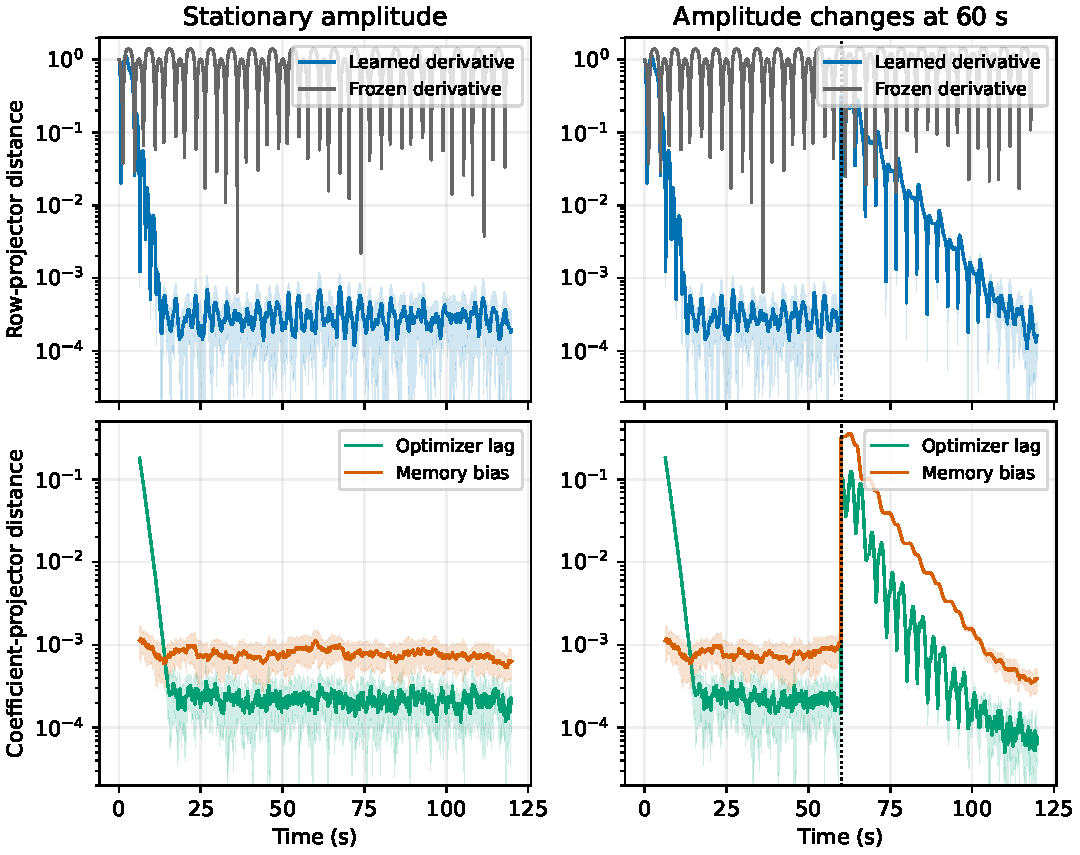
\includegraphics[width=\textwidth]{direct_lift_diagnostics}
 \caption{Direct lifted rate-field learning, all ten seeds per scenario.
 Lines show the across-seed mean and shading shows one sample standard
 deviation, displayed on logarithmic axes. Upper panels compare evaluated
 row-projector error for the learned and frozen fields. Lower panels
 separate coefficient optimization lag from empirical-memory bias.
 The vertical dotted line marks the amplitude change. Lower panels begin
 after one phase cycle; every fifth sample is displayed, while all samples
 in the declared windows enter the statistics.}
 \label{fig:direct_lift_diagnostics}
\end{figure*}

Table~\ref{tab:direct_lift_results} reports time means for each seed and
then mean $\pm$ sample standard deviation across all ten seeds. In
$[100,120)$~s, the learned physical row-projector error is
$(2.940\pm0.320)\times10^{-4}$ for the stationary case and
$(5.187\pm0.744)\times10^{-4}$ after the jump. In the jump window
$[60,80)$~s it is $(9.330\pm0.007)\times10^{-2}$: the estimator does
not instantaneously acquire the changed derivative. In the same window,
the coefficient memory bias exceeds the optimizer lag, consistent with
retaining incompatible pre-change data. These are observations for this
protocol, not a theorem about arbitrary changes or noise models.

Across all recorded samples and seeds, the minimum evaluated row norm is
0.670324 for the stationary case and 0.529792 for the jump case; no
zero-row or nonfinite projector was observed. The maximum coefficient
unit-norm deviation is $3.34\times10^{-16}$, rounded upward. No
increase in the frozen-memory quadratic energy was recorded during an
adaptation step. These sampled checks do not turn coefficient
normalization into a general phase-uniform rank certificate.

The public postprocessor \path{experiments/plot_direct_lift_audit.py}
independently checked the original file hashes, reconstructed all
120,020 recorded rows from the twenty runs, rebuilt every stored moment,
and recomputed the reported field projectors, energies, norms, and
window statistics. It also checked 280 fixed-index transitions using
direct matrix exponentials, independently of the simulation's spectral
implementation. Raw records, protocol, source snapshot, environment,
and hashes remain a separately identified reproduction artifact; the
supplement contains only the generated figure and table.

This experiment supports direct adaptation of an evaluated differential
row space from tangent observations without derivative-entry targets.
Its scope remains a known harmonic basis, exact clock/phase, one initial
coefficient row, one stationary amplitude and one prescribed jump, and
sensor-noise variation. It does not establish frequency discovery,
generalization to unrelated trajectories, or closed-loop performance.

\subsection{Exact-Jacobian companion with every coefficient adaptive}
\label{sec:direct_jacobian_companion}
A separately declared companion, \texttt{direct\_jacobian\_20261118\_v1},
tests the additional integrability restriction that every candidate row be
an exact Jacobian, not just a rate-product field. This is a different
restriction from direct learning without supplied physical partial algebra;
its prescribed residual family is
\begin{align}
 f_q(x,y)&=q_0x+q_1y+q_2\sin x+q_3\cos x,\\
 F_q(x,y)&=(q_0+q_2\cos x-q_3\sin x,\ q_1),
 \label{eq:direct_jacobian_family}\\
 \psi_J&=\col(v_1,v_2,\cos x\,v_1,-\sin x\,v_1).
\end{align}
All four coefficients adapt, including $q_1$; no derivative entry is
held at its true value. The clock rate $v_1=1$ is an observed context
channel, not a fixed learned derivative coefficient. The learner uses
$q\psi_J=F_qv_m$ and the same normalized update
(\ref{eq:direct_step}), with a $4\times4$ memory. It receives no residual
level and no derivative-entry targets. The derivative is exact at fixed
$q$ for every iterate; an adapting residual still has the parameter term
in its total time derivative.
After the jump, the continuous physical level in
(\ref{eq:direct_piecewise_level}) includes the additive offset
$(A_1-A_2)\sin x_c$. That constant is absent from this candidate basis,
is not learned, and is not used: its derivative is zero, so the physical
Jacobian remains representable on each segment.

The stationary/jump schedules, step, memory, gain, noise, durations, and
twenty seed/scenario combinations are unchanged. The separately fixed
initial row is $(0.3,1,-0.3,0.2)$ normalized to unit length. This
four-dimensional family and initialization were declared before its runs;
the six-dimensional protocol and records were preserved. A trace-level
comparison confirmed that all twenty tangent observation streams match
their six-dimensional counterparts exactly. The families have different
constraints and initial rows, so their numerical differences are not a
comparison of estimators with matched capacity.

\begin{directproposition}[Exact Jacobians and clean identifiability]
\label{prop:direct_jacobian_identifiability}
For every $q\in\mathbb R^4$, (\ref{eq:direct_jacobian_family}) is
$D_zf_q$ and $q\psi_J=F_qv$. For every constant real $A$, the
clean full-period covariance of $\psi_J$ has eigenvalues
\begin{equation}
 \{0,\tfrac12,1,\tfrac{1+A^2}{2}\}
\end{equation}
and its kernel is spanned by $(0,1,A,0)$.
\end{directproposition}
\begin{IEEEproof}
Differentiate $f_q$ with respect to $x$ and $y$ while holding $q$ fixed;
substitution gives the tangent-product identity. With
$v=(1,-A\cos x)$, the clean incompatibility is
$q_0+(q_2-Aq_1)\cos x-q_3\sin x$.
Independence of these three harmonics gives the stated kernel.
The constant and sine coordinates have covariance eigenvalues $1$ and
$1/2$. The remaining block is
$\frac12\left[\begin{smallmatrix}A^2&-A\\-A&1\end{smallmatrix}\right]$,
whose eigenvalues are $0$ and $(1+A^2)/2$.
\end{IEEEproof}
Unlike the larger rate-field family, the exact-Jacobian family retains a
one-dimensional clean kernel even at $A=0$. This difference comes from
the integrability restriction and smaller candidate space. It does not
establish robustness for arbitrary features or sensing assumptions.

\begin{table*}[t]
\centering
\caption{Exact-Jacobian companion: mean $\pm$ sample standard deviation across all ten seeds per scenario, after averaging each pre-update diagnostic over its half-open time window. Every candidate is an exact Jacobian and all four coefficients adapt.}
\label{tab:direct_jacobian_results}
\begin{tabular}{llcccc}
\toprule
Scenario & Window (s) & Learned derivative & Frozen derivative & Optimizer lag & Memory bias\\
\midrule
Stationary & 40--60 & $(2.479\pm0.728)\times10^{-4}$ & $(9.075\pm0.000)\times10^{-1}$ & $(4.123\pm0.266)\times10^{-5}$ & $(3.373\pm1.061)\times10^{-4}$\\
Stationary & 60--80 & $(2.529\pm0.693)\times10^{-4}$ & $(9.022\pm0.000)\times10^{-1}$ & $(4.163\pm0.365)\times10^{-5}$ & $(3.244\pm0.890)\times10^{-4}$\\
Stationary & 100--120 & $(2.631\pm0.456)\times10^{-4}$ & $(8.870\pm0.000)\times10^{-1}$ & $(4.108\pm0.320)\times10^{-5}$ & $(3.553\pm0.592)\times10^{-4}$\\
\midrule
Jump & 40--60 & $(2.479\pm0.728)\times10^{-4}$ & $(9.075\pm0.000)\times10^{-1}$ & $(4.123\pm0.266)\times10^{-5}$ & $(3.373\pm1.061)\times10^{-4}$\\
Jump & 60--80 & $(8.872\pm0.007)\times10^{-2}$ & $(1.042\pm0.000)\times10^{0}$ & $(3.974\pm0.004)\times10^{-3}$ & $(9.678\pm0.008)\times10^{-2}$\\
Jump & 100--120 & $(4.825\pm0.712)\times10^{-4}$ & $(1.034\pm0.000)\times10^{0}$ & $(3.476\pm0.253)\times10^{-5}$ & $(5.290\pm0.596)\times10^{-4}$\\
\bottomrule
\end{tabular}
\end{table*}

All twenty companion runs and all 120,020 recorded rows were audited
independently, including complete memory reconstruction and another
280 transitions checked with direct matrix exponentials. Three focused
tests additionally check finite-difference Jacobians for arbitrary
coefficients, the covariance spectrum, and the tangent-feature identity.
The minimum evaluated row norm over every seed and sample is 0.509438;
no invalid row projector or frozen-memory energy increase was recorded,
and the largest unit-norm deviation is $2.23\times10^{-16}$, rounded up.

The learned physical row-projector error in $[100,120)$~s is
$(2.631\pm0.456)\times10^{-4}$ for the stationary case and
$(4.825\pm0.712)\times10^{-4}$ after the jump. During $[60,80)$~s
after the jump it is $(8.872\pm0.007)\times10^{-2}$.
Table~\ref{tab:direct_jacobian_results} includes the frozen baseline,
optimizer lag, and empirical-memory bias using the same gauge-invariant
definitions as above. Thus this companion supplies numerical evidence of
coefficient-induced Jacobian row-space recovery within its prescribed
family, with every coefficient adaptive and every candidate integrable.
It is not independent-entry partial learning with unknown algebraic structure.
The evidence remains confined to the declared family, observations,
initialization, and two amplitude schedules. Additive levels remain
unidentified, and no control or generalization claim is added.
